\section{Producto punto}

Hasta ahora se ha explorado la multiplicación escalar, donde al multiplicar un vector por un valor escalar se obtiene como resultado otro vector. Sin embargo, en el álgebra vectorial es posible multiplicar dos vectores entre sí. 

Existen dos formas principales de multiplicar vectores en cálculo multivariable. La primera de ellas es el \textbf{producto punto}, también conocido como \textbf{producto escalar} o \textbf{producto interno}. Su principal característica es que la operación toma dos vectores y devuelve como resultado un valor escalar, no un vector.

En aplicaciones de ingeniería y física, el producto punto es una herramienta indispensable. Permite determinar de forma cuantitativa qué tanto "apuntan" dos vectores en la misma dirección, calcular el trabajo mecánico realizado por una fuerza a lo largo de un desplazamiento, o encontrar las proyecciones de un vector sobre otro.

\subsubsection{Definición Algebraica en $\mathbb{R}^n$}

Desde el punto de vista algebraico, el producto punto es una operación muy directa. Se calcula simplemente multiplicando las componentes correspondientes de ambos vectores y luego sumando esos resultados parciales.

\begin{mydefinition}{Producto Punto en $\mathbb{R}^n$}
Sean $\vec{u} = (u_1, u_2, \dots, u_n)$ y $\vec{v} = (v_1, v_2, \dots, v_n)$ dos vectores en el espacio euclidiano $\mathbb{R}^n$. El producto punto de $\vec{u}$ y $\vec{v}$, denotado por el símbolo de un punto centrado $\vec{u} \cdot \vec{v}$, se define como el escalar resultante de:
\[ \vec{u} \cdot \vec{v} = u_1v_1 + u_2v_2 + \dots + u_nv_n \]

De forma compacta, utilizando la notación de sumatoria, se expresa como:
\[ \vec{u} \cdot \vec{v} = \sum_{i=1}^{n} u_i v_i \]
\end{mydefinition}

\subsubsection{Propiedades del Producto Punto}

Al igual que las operaciones aritméticas básicas, el producto punto obedece a ciertas leyes algebraicas que nos permiten manipular y simplificar ecuaciones vectoriales. Sean $\vec{u}$, $\vec{v}$ y $\vec{w}$ vectores en $\mathbb{R}^n$, y sea $c$ un escalar. Se cumplen las siguientes propiedades:

\begin{mytheorem}{Propiedades Algebraicas del Producto Punto}
\begin{enumerate}
    \item \textbf{Conmutatividad:} $\vec{u} \cdot \vec{v} = \vec{v} \cdot \vec{u}$
    \item \textbf{Distributividad sobre la suma:} $\vec{u} \cdot (\vec{v} + \vec{w}) = \vec{u} \cdot \vec{v} + \vec{u} \cdot \vec{w}$
    \item \textbf{Asociatividad con un escalar:} $c(\vec{u} \cdot \vec{v}) = (c\vec{u}) \cdot \vec{v} = \vec{u} \cdot (c\vec{v})$
    \item \textbf{Propiedad del vector cero:} $\vec{0} \cdot \vec{v} = 0$
    \item \textbf{Relación con la magnitud:} El producto punto de un vector consigo mismo es igual al cuadrado de su magnitud:
    \[ \vec{v} \cdot \vec{v} = \|\vec{v}\|^2 \quad \text{o bien} \quad \|\vec{v}\| = \sqrt{\vec{v} \cdot \vec{v}} \]
\end{enumerate}
\end{mytheorem}

\subsection{Ángulo entre Dos Vectores}

Aunque definimos el producto punto de forma algebraica multiplicando componentes, su verdadera utilidad en ingeniería y física radica en su interpretación geométrica. El producto punto nos revela la relación angular entre dos vectores.

Si colocamos dos vectores $\vec{u}$ y $\vec{v}$ de modo que compartan el mismo origen, estos formarán un ángulo $\theta$ entre ellos, donde $0 \leq \theta \leq \pi$.

\begin{mytheorem}{Ángulo entre vectores}
Si $\theta$ es el ángulo entre dos vectores no nulos $\vec{u}$ y $\vec{v}$, entonces el producto punto está dado geométricamente por:
\[ \vec{u} \cdot \vec{v} = \|\vec{u}\| \|\vec{v}\| \cos(\theta) \]

De esta fórmula se puede despejar el ángulo $\theta$ para calcularlo a partir de las componentes de los vectores:
\[ \cos(\theta) = \frac{\vec{u} \cdot \vec{v}}{\|\vec{u}\| \|\vec{v}\|} \]
\end{mytheorem}

\subsubsection{Visualización y Demostración}

Para demostrar este teorema, se utilizará la geometría del triángulo formado por los vectores y se aplicará la \textbf{Ley de los Cosenos}.

\begin{center}
\shorthandoff{>}
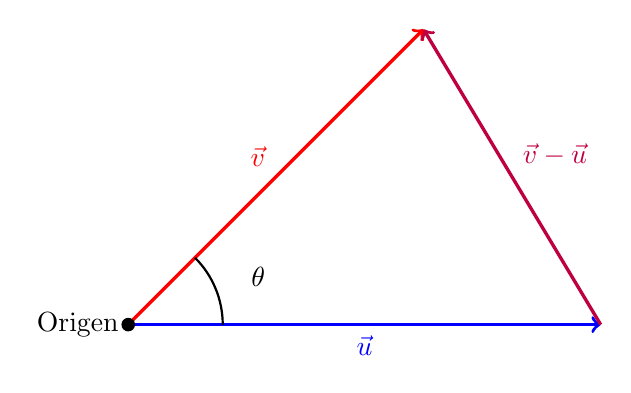
\begin{tikzpicture}[scale=1.5]
    % Vectores
    \draw[->, very thick, blue] (0,0) -- (4,0) node[midway, below] {$\vec{u}$};
    \draw[->, very thick, red] (0,0) -- (2.5,2.5) node[midway, above left] {$\vec{v}$};
    
    % Vector diferencia cerrando el triángulo
    \draw[->, very thick, purple] (4,0) -- (2.5,2.5) node[midway, above right] {$\vec{v} - \vec{u}$};
    
    % Ángulo theta
    \draw[thick] (0.8,0) arc (0:45:0.8);
    \node at (1.1,0.4) {$\theta$};
    
    % Puntos en los extremos
    \filldraw[black] (0,0) circle (1.5pt) node[left] {Origen};
\end{tikzpicture}
\end{center}

\begin{proof}[Demostración mediante la Ley de los Cosenos]

Considerese un triángulo cuyos lados están formados por los vectores $\vec{u}$, $\vec{v}$ y el vector diferencia $\vec{v} - \vec{u}$. Las longitudes de los lados de este triángulo son exactamente las magnitudes de estos vectores: $\|\vec{u}\|$, $\|\vec{v}\|$ y $\|\vec{v} - \vec{u}\|$.

Aplicando la Ley de los Cosenos a este triángulo para relacionar los lados con el ángulo $\theta$, se tiene:
\[ \|\vec{v} - \vec{u}\|^2 = \|\vec{u}\|^2 + \|\vec{v}\|^2 - 2\|\vec{u}\|\|\vec{v}\|\cos(\theta) \]

Ahora, se reescribe el lado izquierdo de la ecuación utilizando la propiedad que relaciona la magnitud con el producto punto ($\|\vec{x}\|^2 = \vec{x} \cdot \vec{x}$):
\[ \|\vec{v} - \vec{u}\|^2 = (\vec{v} - \vec{u}) \cdot (\vec{v} - \vec{u}) \]

Aplicando la propiedad distributiva del producto punto, se desarrolla este binomio:
\[ (\vec{v} - \vec{u}) \cdot (\vec{v} - \vec{u}) = \vec{v} \cdot \vec{v} - \vec{v} \cdot \vec{u} - \vec{u} \cdot \vec{v} + \vec{u} \cdot \vec{u} \]

Usando la propiedad conmutativa ($\vec{u} \cdot \vec{v} = \vec{v} \cdot \vec{u}$) y convirtiendo de vuelta a magnitudes:
\[ \|\vec{v} - \vec{u}\|^2 = \|\vec{v}\|^2 - 2(\vec{u} \cdot \vec{v}) + \|\vec{u}\|^2 \]

Se iguala esta expresión algebraica con la ecuación geométrica obtenida de la Ley de los Cosenos:
\[ \|\vec{v}\|^2 - 2(\vec{u} \cdot \vec{v}) + \|\vec{u}\|^2 = \|\vec{u}\|^2 + \|\vec{v}\|^2 - 2\|\vec{u}\|\|\vec{v}\|\cos(\theta) \]

Restando $\|\vec{u}\|^2$ y $\|\vec{v}\|^2$ de ambos lados, la ecuación se simplifica notablemente a:
\[ -2(\vec{u} \cdot \vec{v}) = -2\|\vec{u}\|\|\vec{v}\|\cos(\theta) \]

Finalmente, dividiendo ambos lados entre $-2$, se llega a que:
\[ \vec{u} \cdot \vec{v} = \|\vec{u}\|\|\vec{v}\|\cos(\theta) \]
\end{proof}

\subsection{Vectores ortogonales}

Una de las consecuencias más útiles del teorema del ángulo entre dos vectores es que nos proporciona una prueba algebraica para determinar si dos vectores son perpendiculares entre sí.

Si dos vectores no nulos $\vec{u}$ y $\vec{v}$ son ortogonales, el ángulo entre ellos es exactamente $\theta = \frac{\pi}{2}$ radianes. 

Sustituyendo este valor en nuestra fórmula geométrica:
\[ \vec{u} \cdot \vec{v} = \|\vec{u}\|\|\vec{v}\|\cos\left(\frac{\pi}{2}\right) \]

Dado que $\cos(\frac{\pi}{2}) = 0$, toda la expresión de la derecha se anula.

\begin{mytheorem}{Condición de ortogonalidad}
Dos vectores no nulos $\vec{u}$ y $\vec{v}$ son ortogonales si y solo si su producto punto es igual a cero:
\[ \vec{u} \cdot \vec{v} = 0 \]
Por convención matemática, se considera que el vector cero ($\vec{0}$) es ortogonal a cualquier otro vector, ya que $\vec{0} \cdot \vec{v} = 0$ para todo $\vec{v}$.
\end{mytheorem}

\subsection{Cosenos directores}

En el espacio $\mathbb{R}^3$, a menudo es necesario describir la dirección exacta de un vector en relación con el sistema de coordenadas. Para ello, se utilizan los \textbf{ángulos directores} $\alpha$, $\beta$ y $\gamma$, que son los ángulos que el vector forma con los ejes positivos $x$, $y$ y $z$, respectivamente.

Si se toma un vector $\vec{v} = (v_1, v_2, v_3)$ y se calcula el producto punto de este vector con cada uno de los vectores unitarios canónicos ($\hat{i}, \hat{j}, \hat{k}$), es posible encontrar los cosenos de estos ángulos, conocidos como \textbf{cosenos directores}.

Por ejemplo, para el ángulo $\alpha$ con el eje $x$:
\[ \vec{v} \cdot \hat{\imath} = \|\vec{v}\|\|\hat{\imath}\|\cos(\alpha) \]
Sabiendo que $\vec{v} \cdot \hat{\imath} = (v_1)(1) + (v_2)(0) + (v_3)(0) = v_1$ y que $\|\hat{\imath}\| = 1$, se obtiene:
\[ v_1 = \|\vec{v}\|\cos(\alpha) \implies \cos(\alpha) = \frac{v_1}{\|\vec{v}\|} \]

\begin{mydefinition}{Cosenos directores}
Para cualquier vector no nulo $\vec{v} = (v_1, v_2, v_3)$, sus cosenos directores son:
\[ \cos(\alpha) = \frac{v_1}{\|\vec{v}\|}, \quad \cos(\beta) = \frac{v_2}{\|\vec{v}\|}, \quad \cos(\gamma) = \frac{v_3}{\|\vec{v}\|} \]

Una propiedad importante es que la suma de los cuadrados de los cosenos directores siempre es igual a 1:
\[ \cos^2(\alpha) + \cos^2(\beta) + \cos^2(\gamma) = 1 \]
\end{mydefinition}

Un hecho interesante, es que los cosenos directores son exactamente las componentes del \textbf{vector unitario} que apunta en la dirección de $\vec{v}$. Es decir:
\[ \frac{\vec{v}}{\|\vec{v}\|} = (\cos\alpha, \cos\beta, \cos\gamma) \]

\begin{center}
\shorthandoff{>}
\begin{tikzpicture}[x={(-0.5cm,-0.5cm)}, y={(1cm,0cm)}, z={(0cm,1cm)}, scale=2]
    % Ejes
    \draw[->, gray] (0,0,0) -- (2,0,0) node[below left] {$x$};
    \draw[->, gray] (0,0,0) -- (0,2,0) node[right] {$y$};
    \draw[->, gray] (0,0,0) -- (0,0,2) node[above] {$z$};
    
    % Vector v
    \coordinate (V) at (1.2, 1.5, 1.5);
    \draw[->, very thick, blue] (0,0,0) -- (V) node[above right] {$\vec{v}$};
    
    % Arcos para los ángulos directores
    % Alfa (con el eje x)
    \draw[thick, red] (0.5,0,0) to[out=90,in=-120] (0.4, 0.5, 0.5);
    \node[red, below=2pt] at (0.6, 0.2, 0.2) {$\alpha$};
    
    % Beta (con el eje y)
    \draw[thick, green!60!black] (0,0.6,0) to[out=90,in=-30] (0.3, 0.5, 0.4);
    \node[green!60!black, right=2pt] at (0.2, 0.6, 0.2) {$\beta$};
    
    % Gamma (con el eje z)
    \draw[thick, orange] (0,0,0.6) to[out=0,in=150] (0.3, 0.4, 0.4);
    \node[orange, left=2pt] at (0.1, 0.2, 0.7) {$\gamma$};
\end{tikzpicture}
\end{center}


\subsection{Proyección Vectorial}

Una aplicación práctica del producto punto es averiguar qué parte de un vector actúa exactamente en la misma dirección que otro vector. Imagina que tienes una fuente de luz que brilla directamente sobre un vector $\vec{u}$, perpendicular a un segundo vector $\vec{v}$. La "sombra" que $\vec{u}$ proyecta sobre la línea de acción de $\vec{v}$ es lo que se conoce como \textbf{proyección vectorial}.

\begin{center}
\shorthandoff{>}
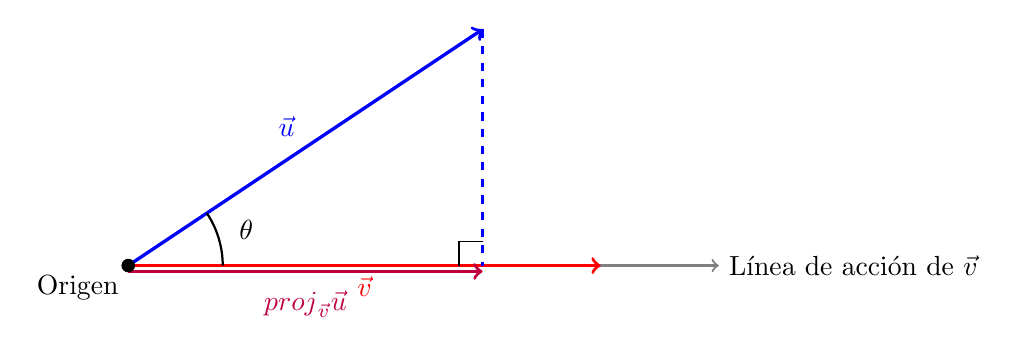
\begin{tikzpicture}[scale=1.5]
    % Línea de acción base
    \draw[->, thick, gray] (0,0) -- (5,0) node[right, black] {Línea de acción de $\vec{v}$};
    \draw[->, very thick, red] (0,0) -- (4,0) node[midway, below] {$\vec{v}$};
    
    % Vector u a proyectar
    \draw[->, very thick, blue] (0,0) -- (3,2) node[midway, above left] {$\vec{u}$};
    
    % Línea de proyección (perpendicular) indicando la "sombra"
    \draw[dashed, thick, blue] (3,2) -- (3,0);
    
    % Símbolo de ángulo recto
    \draw (2.8,0) -- (2.8,0.2) -- (3,0.2);
    
    % Ángulo theta
    \draw[thick] (0.8,0) arc (0:33.69:0.8);
    \node at (1,0.3) {$\theta$};
    
    % Vector Proyección (la "sombra")
    \draw[->, very thick, purple, yshift=-0.05cm] (0,0) -- (3,0) node[midway, below=3pt] {$\text{proj}_{\vec{v}}\vec{u}$};
    
    % Punto de origen
    \filldraw[black] (0,0) circle (1.5pt) node[below left] {Origen};
\end{tikzpicture}
\end{center}

Para encontrar la fórmula matemática de este nuevo vector proyección, $\text{proj}_{\vec{v}}\vec{u}$, debe construirse paso a paso utilizando su geometría. Todo vector requiere dos cosas: una dirección y una magnitud.

\textbf{1. La Dirección:} 
Se sabe que la proyección debe estar sobre la misma línea que el vector $\vec{v}$. Por lo tanto, compartirá su mismo vector unitario direccional.
\[ \text{Dirección} = \frac{\vec{v}}{\|\vec{v}\|} \]

\textbf{2. La Magnitud:} 
Si se observa el triángulo rectángulo formado en el gráfico anterior, la hipotenusa es la magnitud de nuestro vector original ($\|\vec{u}\|$). La longitud de la sombra (nuestra proyección) corresponde al cateto adyacente al ángulo $\theta$. Usando trigonometría básica ($\cos\theta = \frac{\text{adyacente}}{\text{hipotenusa}}$), se tiene que:
\[ \text{Magnitud} = \|\vec{u}\| \cos(\theta) \]

\textbf{3. Construcción del Vector:}
Multiplicando la magnitud por la dirección se obtiene la definición geométrica de la proyección:
\[ \text{proj}_{\vec{v}}\vec{u} = (\|\vec{u}\| \cos\theta) \left(\frac{\vec{v}}{\|\vec{v}\|}\right) \]

Dado que rara vez se conoce el ángulo $\theta$, se puede utilizar la propiedad del producto punto de ángulo entre vectores ($\vec{u} \cdot \vec{v} = \|\vec{u}\|\|\vec{v}\| \cos\theta$) para despejar el término del coseno ($\cos\theta = \frac{\vec{u} \cdot \vec{v}}{\|\vec{u}\|\|\vec{v}\|}$) y sustituirlo en la ecuación:

\[ \text{proj}_{\vec{v}}\vec{u} = \left( \|\vec{u}\| \frac{\vec{u} \cdot \vec{v}}{\|\vec{u}\|\|\vec{v}\|} \right) \frac{\vec{v}}{\|\vec{v}\|} \]

Al simplificar, cancelando $\|\vec{u}\|$ y multiplicando los denominadores, se llega a la fórmula algebraica final que es la que se utiliza para calcular proyecciones en $\mathbb{R}^n$:

\begin{mydefinition}{Proyección Vectorial}
La proyección vectorial de $\vec{u}$ sobre $\vec{v}$ se calcula únicamente usando el producto punto y la magnitud del vector base:
\[ \text{proj}_{\vec{v}}\vec{u} = \left( \frac{\vec{u} \cdot \vec{v}}{\|\vec{v}\|^2} \right) \vec{v} \]
\end{mydefinition}

\subsubsection{Magnitud del vector proyección}

En muchas ocasiones, no es de interés el vector completo resultante de la proyección, sino únicamente su longitud. A esta longitud se le conoce como \textbf{proyección escalar} o \textbf{componente} de $\vec{u}$ a lo largo de $\vec{v}$.

Como se realizó en el desarrollo geométrico, esta magnitud está dada por $\|\vec{u}\| \cos\theta$. Al igual que antes, si sustituimos el coseno utilizando el producto punto, se obtiene su fórmula directa.

\begin{mydefinition}{Proyección Escalar}
La proyección escalar o componente del vector $\vec{u}$ en la dirección del vector $\vec{v}$ se denota como $\text{comp}_{\vec{v}}\vec{u}$ y es un número real definido como:
\[ \text{comp}_{\vec{v}}\vec{u} = \|\vec{u}\| \cos(\theta) = \frac{\vec{u} \cdot \vec{v}}{\|\vec{v}\|} \]
\end{mydefinition}

\textit{Nota:} Aunque se habla de longitud, la componente escalar puede ser un número negativo. Si el ángulo $\theta$ entre los vectores es mayor a $\frac{\pi}{2}$, el coseno será negativo. Geométricamente, esto significa que la proyección sombra está apuntando en la dirección opuesta al vector $\vec{v}$.

\subsection{Ejercicios}

\begin{enumerate}
    \item Calcular el producto punto de cada par de vectores:
\begin{enumerate}
    \item $\vec{u} = (3, -2)$ y $\vec{v} = (1, 4)$
    \item $\vec{a} = (1, -3, 2)$ y $\vec{b} = (4, 1, -2)$
\end{enumerate}
    \item Sea $\vec{v} = (2, -3, 6)$. Verificar la propiedad $\vec{v} \cdot \vec{v} = \|\vec{v}\|^2$ calculando ambos lados de la igualdad por separado.
    \item Sean $\vec{u} = (1, 2, -1)$, $\vec{v} = (3, 0, 2)$ y $c = 4$. Verificar las siguientes propiedades del producto punto usando los valores dados:
\begin{enumerate}
    \item Conmutatividad: $\vec{u} \cdot \vec{v} = \vec{v} \cdot \vec{u}$
    \item Asociatividad con escalar: $c(\vec{u} \cdot \vec{v}) = (c\vec{u}) \cdot \vec{v}$
\end{enumerate}
    \item Determinar cuáles de los siguientes pares de vectores son ortogonales entre sí:
\begin{enumerate}
    \item $\vec{u} = (2, -3)$ y $\vec{v} = (3, 2)$
    \item $\vec{a} = (1, -1, 2)$ y $\vec{b} = (2, 0, -1)$
    \item $\vec{p} = (4, 2, -1)$ y $\vec{q} = (1, -3, -2)$
\end{enumerate}
    \item Encontrar el ángulo $\theta$ (en grados) que forman los siguientes pares de vectores:
\begin{enumerate}
    \item $\vec{u} = (1, 0, 0)$ y $\vec{v} = (1, 1, 0)$
    \item $\vec{a} = (2, -1, 3)$ y $\vec{b} = (1, 2, -1)$
\end{enumerate}
    \item Encontrar el valor o los valores del parámetro $k$ para que los siguientes vectores sean ortogonales:
\begin{enumerate}
    \item $\vec{u} = (k, 3)$ y $\vec{v} = (2, -k)$
    \item $\vec{a} = (1, k, -2)$ y $\vec{b} = (3, -1, k)$
\end{enumerate}
    \item Dado el vector $\vec{v} = (1, 2, -2)$:
\begin{enumerate}
    \item Calcular los ángulos directores $\alpha$, $\beta$ y $\gamma$ (en grados).
    \item Verificar la identidad $\cos^2(\alpha) + \cos^2(\beta) + \cos^2(\gamma) = 1$.
    \item Escribir el vector unitario en la dirección de $\vec{v}$ en términos de sus cosenos directores.
\end{enumerate}
    \item Sean $\vec{u} = (2, 3, -1)$ y $\vec{v} = (4, -1, 2)$. Calcular:
\begin{enumerate}
    \item La proyección escalar $\text{comp}_{\vec{v}}\vec{u}$.
    \item La proyección vectorial $\text{proj}_{\vec{v}}\vec{u}$.
\end{enumerate}
    \item Dado $\vec{u} = (1, -2, 3)$ y $\vec{v} = (2, 1, 1)$, descomponer $\vec{u}$ en dos componentes: una paralela a $\vec{v}$ y otra perpendicular a $\vec{v}$, de modo que:
\[ \vec{u} = \vec{u}_{\parallel} + \vec{u}_{\perp} \]
Verificar que $\vec{u}_\perp \cdot \vec{v} = 0$.
    \item Una fuerza $\vec{F} = (3, -2, 5)$ N actúa sobre un objeto que se desplaza del punto $A = (1, 0, -1)$ al punto $B = (4, 2, 3)$ (distancias en metros).
\begin{enumerate}
    \item Encontrar el vector desplazamiento $\vec{d} = \overrightarrow{AB}$.
    \item Calcular el trabajo $W = \vec{F} \cdot \vec{d}$ realizado por la fuerza (en joules).
    \item Determinar el ángulo que forma la fuerza con el desplazamiento.
\end{enumerate}
    \item Demostrar algebraicamente, usando la definición componente a componente, la propiedad distributiva del producto punto para vectores en $\mathbb{R}^n$:
\[ \vec{u} \cdot (\vec{v} + \vec{w}) = \vec{u} \cdot \vec{v} + \vec{u} \cdot \vec{w} \]
Usar la demostración para verificar con $\vec{u} = (1,2,-1)$, $\vec{v} = (3,0,1)$, $\vec{w} = (-1,2,4)$.
    \item Un sensor de temperatura está ubicado en el punto $P = (2, 1, 3)$. El gradiente de temperatura en ese punto apunta en la dirección $\vec{g} = (4, -2, 1)$. Un robot puede moverse en cualquiera de las siguientes tres direcciones:
\[ \vec{d}_1 = (1, 2, -1), \quad \vec{d}_2 = (-1, 3, 2), \quad \vec{d}_3 = (2, 0, -3) \]
\begin{enumerate}
    \item Calcular la proyección escalar del gradiente sobre cada dirección de movimiento posible.
    \item ¿En qué dirección debe moverse el robot para maximizar el incremento de temperatura? ¿Y para minimizarlo?
\end{enumerate}
\end{enumerate}